\documentclass[10pt]{article}
\usepackage{lipsum}  % For dummy text
\usepackage{graphicx}  % For including images
\usepackage{amsmath}  % For mathematical equations
\usepackage{adjustbox}
\title{Regression Project}
\author{Dylan Kasanders}
\date{\today}

\begin{document}

\maketitle

\begin{abstract}
We fit a linear regression model to predict the median house value for housing blocks in California using a variety of characteristics of the 
housing block including geographical location, housing characteristics, and economic factors. 
The regression on the features obtained a $R^2$ of $0.5443$, and the feature set has strong indiciation that they are related in 
predicting the median house value in California. This linear regression model serves as a foundation for understanding key factors that 
influnece house prices in California, and provides room for improvement with the feature set and parameterization. 
\end{abstract}

\section{Introduction}
Housing prices are a critical aspect of the real estate market, influencing economic planning and individual financial decisions. Having strong predictors for house value can provide valuable insight for a wide range of stakeholders, including policymakers, real estate developers, city planners, and future homeowners. In this report, we aim to develop a linear regression model to explore various variables and their influence on house value. This study uses a dataset from "Sparse Spatial Autoregressions" by Pace R. Kelly and Ronald Barry.\\ 
\hspace*{2em} This dataset is pulled from 1990 U.S. Census data of California, and encompasses features of housing blocks in California. Each data point in the dataset represents a housing block within California. On top of median house value for the block, it also includes variables such as geographical coordinates, total number of rooms and bathrooms in the block, number of residents in the block, median income of the block, and number of households defined as a group of people residing within a home unit. Our objective is to pull out variables of interest from the feature set to identify relationships with median house value. Addtionally, we use the distance the housing block has to both Los Angeles and San Francisco to see if there is a relationship between the distance from these cities and housing price.\\
\hspace*{2em} A moviation for this regression model is to identify variables affecting housing prices within California. By doing this, we are able to find variables of interest for future linear models predicting housing price. With measuring distance from Los Angeles and San Francisco, we hope to explore the relationship between house value and the distance from major cities in that area. More accurate predictor variables will lead to the construction of linear regression models with reduced standard error and thus tighter confidence intervals for housing prices, offering more reliable estimates for market assessment. 


\section{Methodology}
In this report, we aim to develop a linear regression model that predicts the median house value for housing blocks in California 
using a diverse set of variables. 
The variables chosen for this analysis are distinct from each other and capture different aspects that may influence housing prices. The first variable
of interest in the model is a combined weighted distance between the cities Los Angeles and San Francisco ($X_{dist}$). Looking at a heatmap of 
housing values in California,
we can notice an increase in house values that are near Los Angeles and San Francisco. This increase in house value near these two cities
calls for a parameter that can measure the closeness to these two respective cities.
\begin{center}
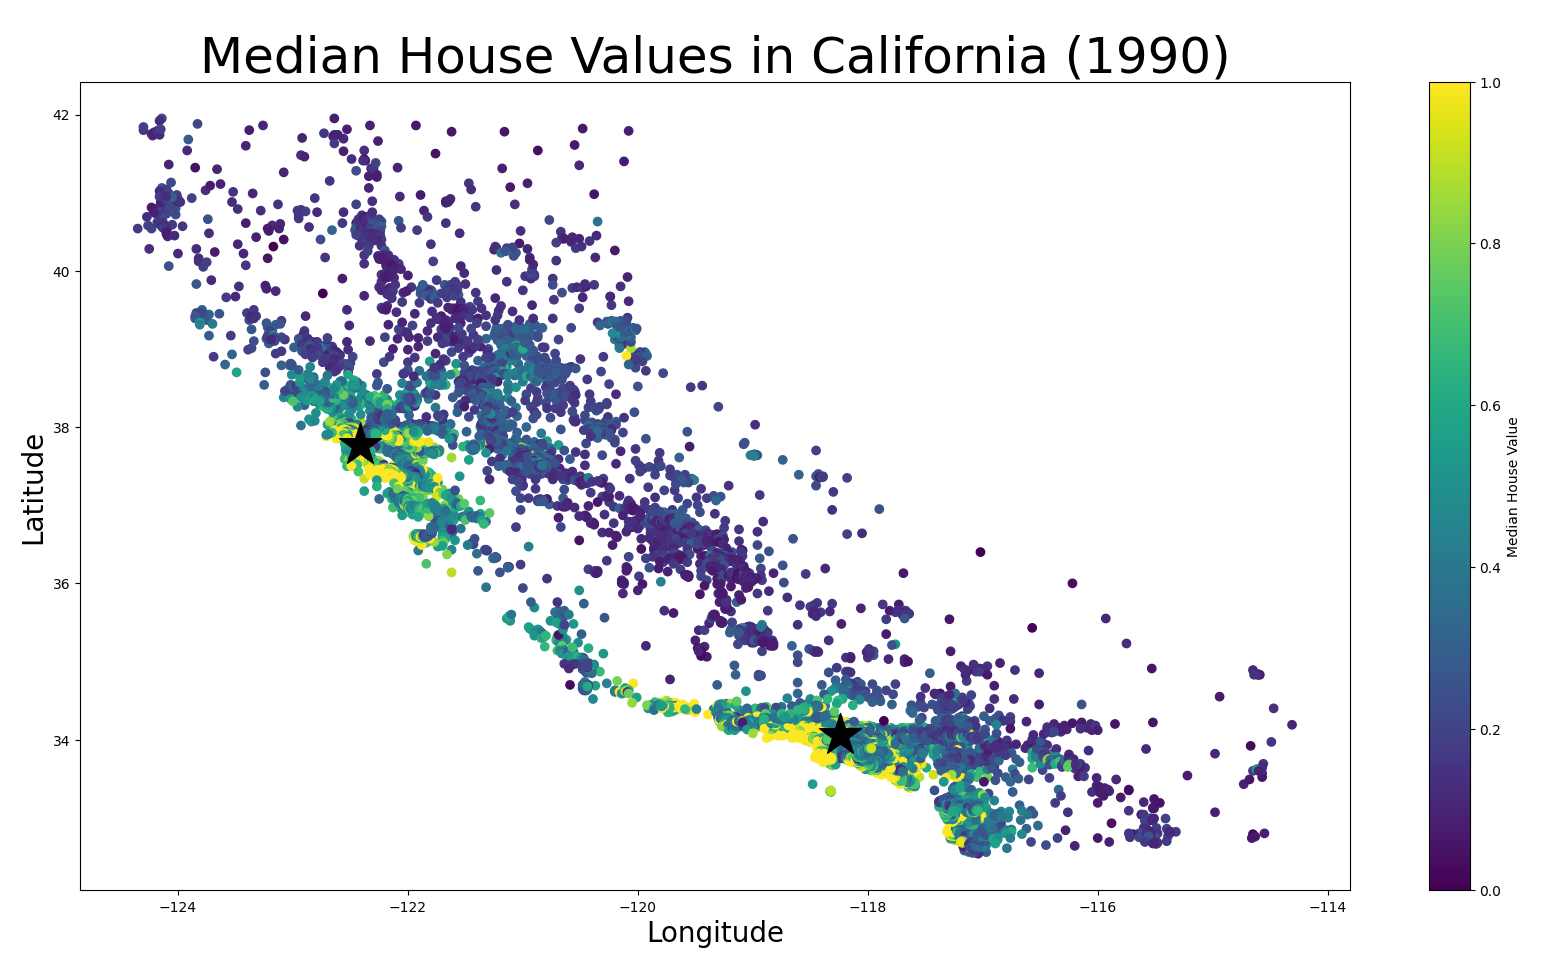
\includegraphics[scale=0.35]{Figure_1}
\end{center}



This regression model uses a weighted distance variable between both Los Angeles and San Francisco to caputre the closeness to either of these cities.
Having a singular variable that measures distance between these two cities addresses the issue of overlap that would occur
using separate distance variables for Los Angeles and San Francisco. By using a singular weighted distance
mesaure, we encapsulate a closeness to either city. Our formula for this weighted distance is defined as:\\
\begin{center}
    $X_{dist}(d_1, d_2) = e^{-d_1} + e^{-d_2}$
\end{center}
\hspace*{2em} Where $d_1$ is the block's distance from Los Angeles, and $d_2$ is the distance from San Francisco.\\
\hspace*{2em} This model also uses extracted features from the dataset to explore their relationship with median house value. 
We construct a variable representing the number of people per household ($X_{PPH}$), 
defined by the ratio between the total population and number of households. 
Total block income ($X_{TBI}$), which is defined as the product between the median income
and population within a block. This variable is used to guage total ecomonic value a block has. 
We also use median income alone in this model ($X_{MI}$). 
We define rooms per household ($X_{RPH}$) as the ratio between the number of rooms and the number of households. 
Bedrooms per room ($X_{BPR}$) is defined as the ratio between the total number of bedrooms and total number of rooms. 
Using these features, we construct a linear regression model:\\
\begin{center}
    $Y_i = \beta_0 + \beta_1X_{dist,i} + \beta_2X_{PPH,i} + \beta_3X_{TBI,i} + \beta_4X_{MI,i} + \beta_5X_{RPH,i} + \beta_6X_{BPR,i} + \epsilon_i$
\end{center}
\hspace*{2em} Note that $X_{dist}$ has an exponential relationship with the predicted value. This implies that as you get closer to either of these cities,
there is an exponential increase in the median house value. This exponential growth emphasises the desireability to be within 
or extremely close to either of these cities
not just near them. There is high desireability to live in an urban city, with factors such as amenities, job opporunities, and better infastructure.
By modeling this relationship exponetially we capture the impact of living within or extremely close to a major city, and thus the price
for purchasing property in the area.\\
\hspace*{2em} Additionally, it's worth noting that during the preprocessing phase, there was an abnormal amount of the maximum value for median house value (\$500,001) which appeared anomalous.
This clustering
suggests a potential issue with the collection of the data or rounding, where values exceeding a threshold have been capped to \$500,001. This anomaly
can distort the linear model and skew the analysis, and thus all points with this median house value have been excluded from the dataset to ensure
the validity of the regression model. This leaves our data having a sample size of $n = 19675$.


\section{Results}
Running this model, we obtained the following coefficients:\\\\
\begin{center}
\begin{adjustbox}{scale=1}
    \begin{tabular}{|c|c|c|c|c|}
        \hline
        Coefficient & Estimate & Standard Error & t Value & $P(>|t|)$\\
        \hline
        Intercept & $8.22e+04$ & $3.871e+03$ & -22.787 & $< 2e-16$ \\
        \hline
        $X_{dist}$ & $9.912e+04$ & $1.812e+03$ & 54.703 & $< 2e-16$ \\
        \hline
        Population Per Household & $-3.417e+02$ & 4.456 & -7.667 & $1.84e-14$\\
        \hline
        Total Block Income & $-3.421e+02$ & $9.738e-02$ & -3.513 & 0.000444\\
        \hline
        Rooms Per Household & $6.95e+02$ & $2.322e+02$ & 2.993 & 0.00277 \\
        \hline
        Bedrooms Per Room & $2.991e+05$ & $1.181e+04$ & 25.324 & $< 2e-16$ \\
        \hline
        Median Income & $4.458e+04$ & $4.447e+02$ & 100.246 & $< 2e-16$\\
        \hline
    \end{tabular}
\end{adjustbox}
\end{center}

\hspace*{2em} With these coefficients, we note that our distance variable, rooms per household, bedrooms per room, 
and median income have a positive relationship with median house value, 
while population per household and total block income have a negative relationship with median house value. Total income block 
having a negative relationship with median house value goes against the initial guiding idea for what total income block was intended to represent,
which was the total income the entire block brings in. We would expect the more income a block has in total, the higher the house values would be.
One reason the coefficient for total block income is negative could be attributed to population exerting a strong influence on the variable.
Given the negative relationship observed between population per household and median house value, there seems to be a negative relationship between
population and house value. This suggests that while higher median incomes in a block are associated with higher housing values, the presence
of a large population within the block doesn't cause a proportional increase in income.\\
\hspace*{2em} The linear regression model notes that each variable selected for the model is significant (with p-values $< 0.05$) in predicting
the mean house value in a block. This signifies that the variables chosen are related to the median house value, and are all worth further consideration
for further understanding on how these variables influence median house value and potential causes for this relationship.\\ 
\hspace*{2em} The linear model has a $R^2$ value of $0.5443$, and a residual standard error of $65970$. The median house value in the dataset
has a standard deviation of $97711.51$. This notes room for improvement in adjusting the model for utilizing the model for constructing
confidence intervals for predicting house values.\\
\hspace*{2em} The linear regression produces the following ANOVA table:\\
\begin{center}
\begin{adjustbox}{scale=1}
    \begin{tabular}{|c|c|c|c|c|}
        \hline
        Source & df & SS & MS & F \\
        \hline
        Regression & 6  & $1.011781e+14$ & $1.686301e+13$ & 3826.956\\
        \hline
        Residual Error & 19667 & $8.666022e+13$ & $4406377182$ & \\
        \hline
        Total & 19674 & $1.878383e+14$ &  & \\
        \hline
    \end{tabular}
\end{adjustbox}
\end{center}
\hspace*{2em} This F-test produces a p-value $< 2.2e-16$, concluding strongly that the variables are predictors for the median house value.\\
\begin{center}
    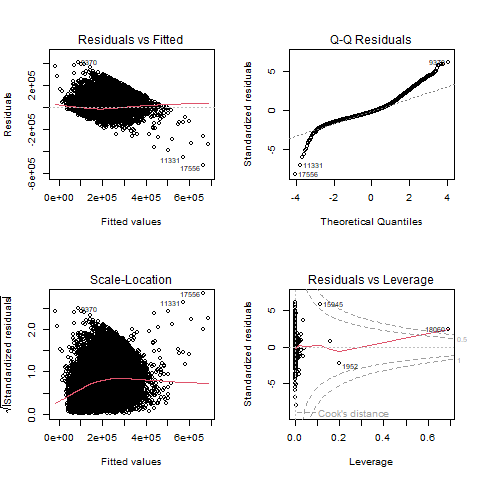
\includegraphics[scale=0.75]{residual}
\end{center}
\hspace*{2em} The linear regression model notes 799 points as influental. Looking at the residuals vs leverage plot, we notice points $18060$ and 
$15945$ have high Cook's distance. Looking at the characteristics of these points, we observe:\\

\begin{tabular}{|c|c|c|}
    \hline
     Point & 18060 & 15945 \\
    \hline
     $Y$ & 137500 & 350000\\
    \hline
     $\hat{Y}$ & 177290.1 & 16100 \\
    \hline
     Combined Distance & 0.4999 & 0.1129 \\
    \hline
     Population Per Household & 1243.333 & 502.4615\\
    \hline
     Total Block Income & 76288.94 & 27851.79 \\
    \hline
     Rooms Per Household & 3.1666 & 9.0769 \\
    \hline
     Bedrooms Per Room & 0.2631 & 0.144\\
    \hline
     Median Income & 10.2264 & 4.2639\\
    \hline
\end{tabular}
\\ \hspace*{2em}Point $18060$ is an outlier due to it's high median income compared to the mean and standard deviation of median income ($3.6767$, $1.5702$ respectively),
while point $15945$ is an outlier due to it's high rooms per household value compared to it's mean and standard deviation ($5.36$, $2.292$). With 799 points being marked as 
influental ($4.06\%$), it's hard to argue that these points are abnormalities or outliers to the housing demographics of California. This speaks to the complex
nature of housing, and the numerous factors that impact the price.\\

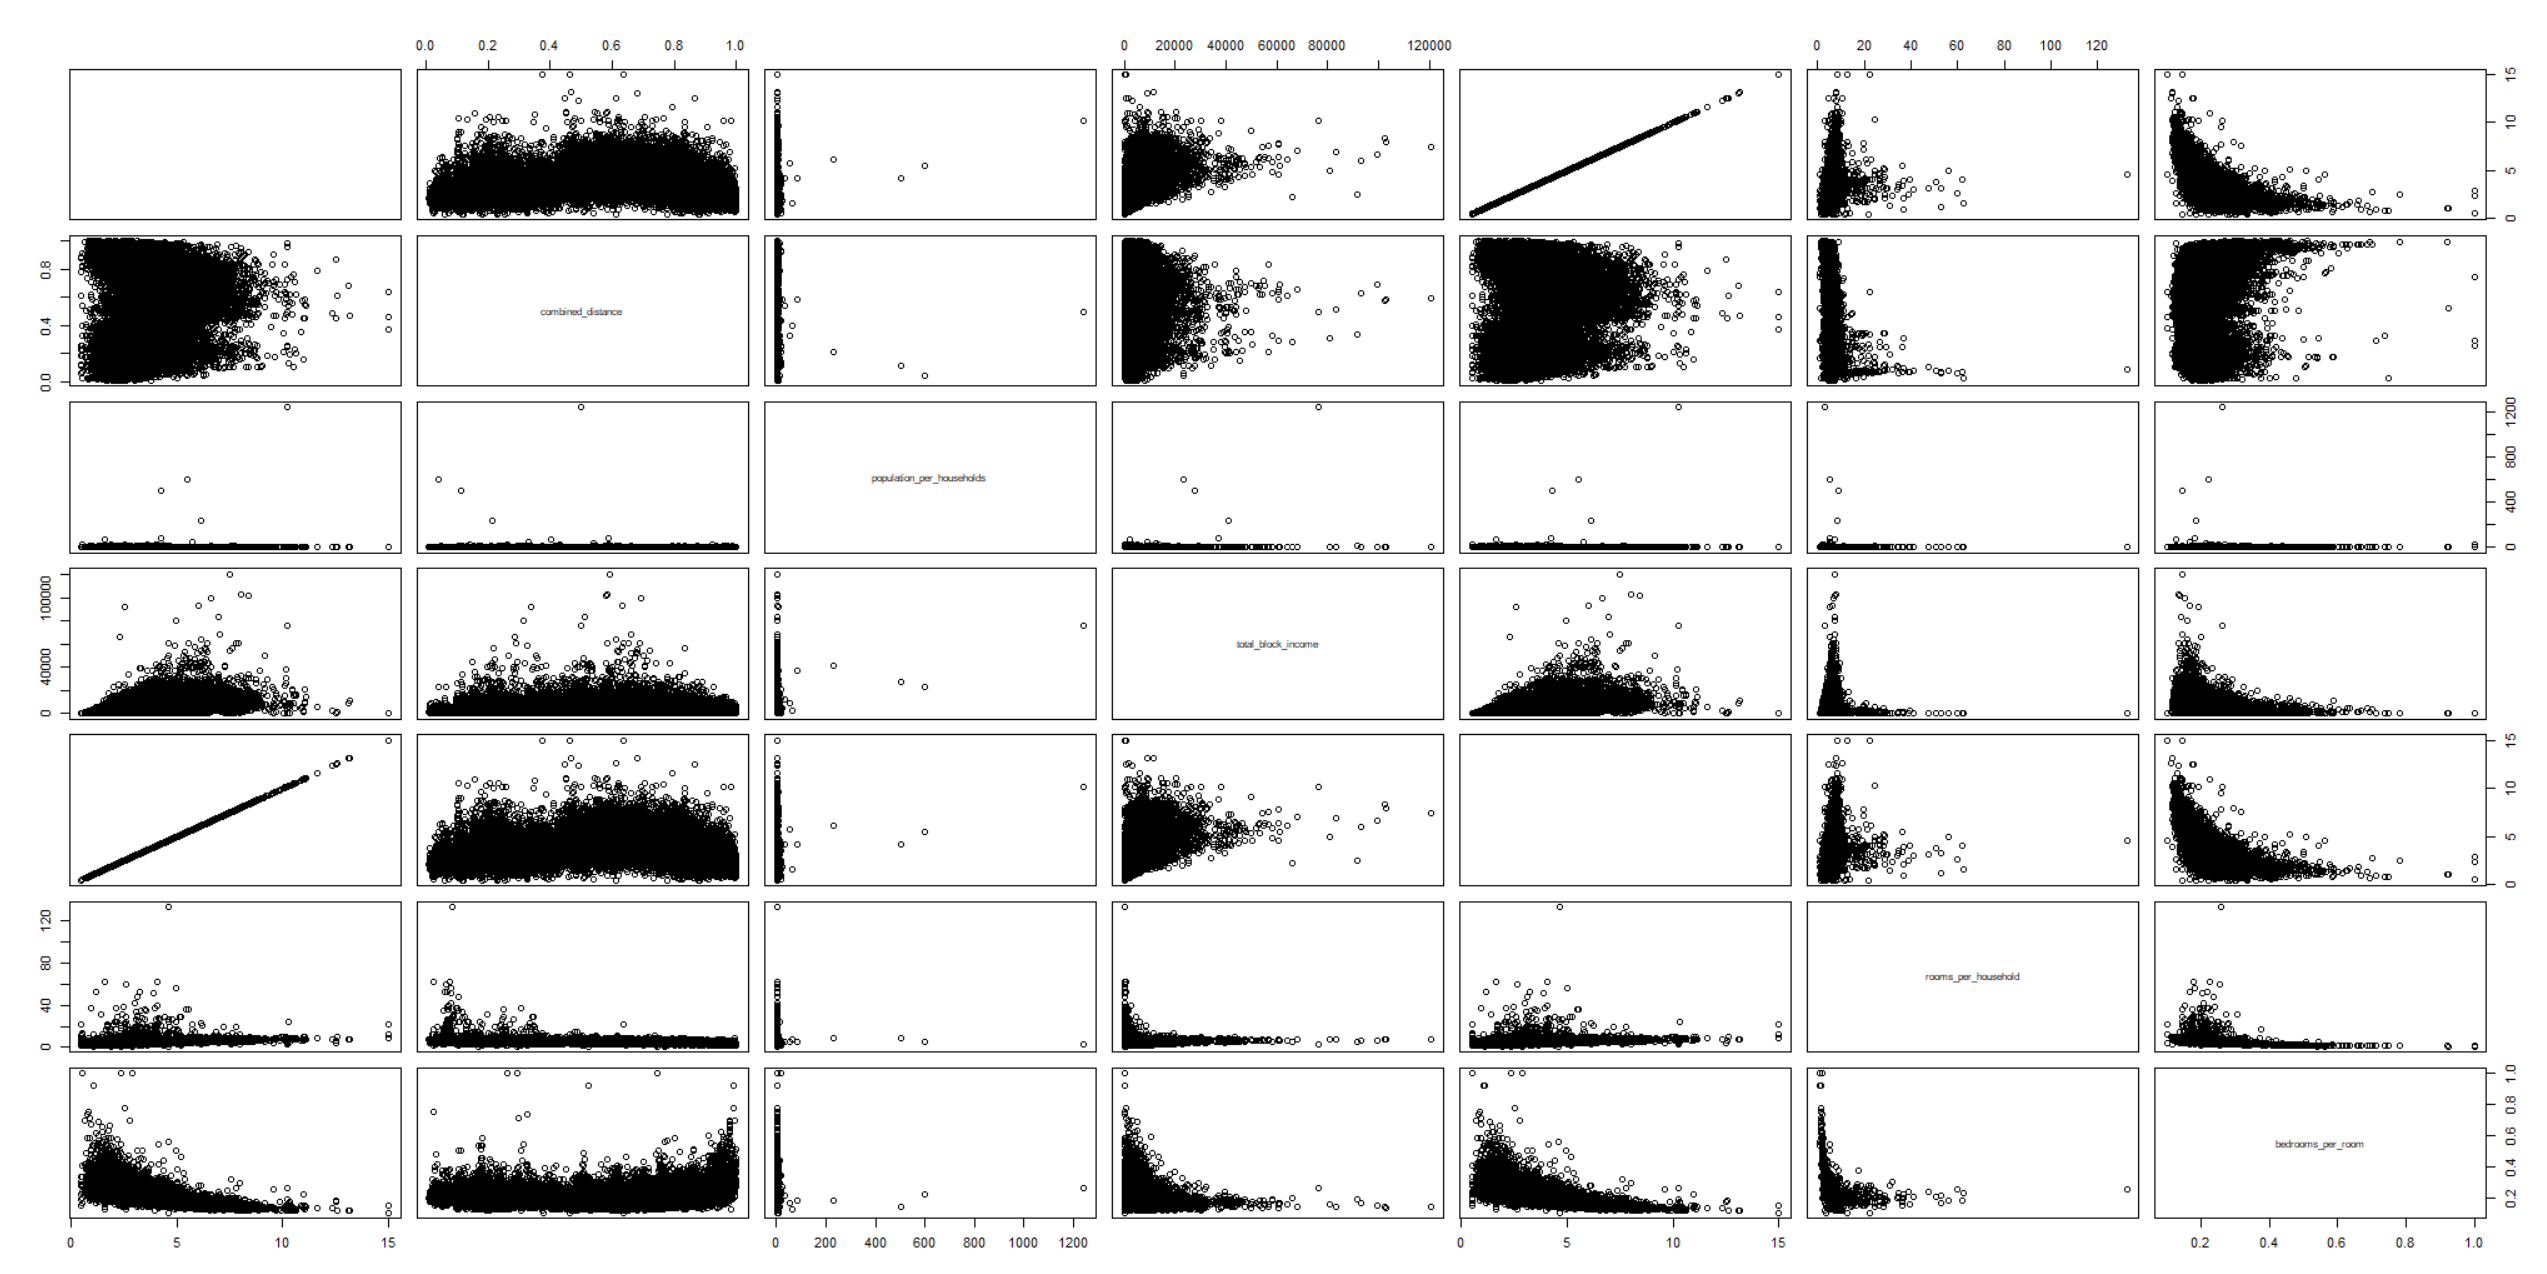
\includegraphics[scale=0.25]{matrix}



\section{Conclusion}
Our regression model aimed to uncover factors influencing median house values in California housing blocks. By utilizing a wide range of variables including
geographical proxmity, demographic characteristics, and economic factors, we constructed a model to explore the impact these factors have on 
median house value. This linear regression model showcases the impact these factors have in predicting median house value. Further engineering and
exploration of these factors is crucial in gaining better understanding of the factors behind median house value.\\
\hspace*{2em} The linear regression model obtained reasonable explanatory power, indicated by an $R^2$ value of $0.5443$. There does remain
room for refinement and future feature engineering and extracting to further predictive accuracy for future use cases of constructing confidence
intervals for housing prices.\\
\hspace*{2em} Our regression analysis offers valuable insights into the determining factors of median house values in California, providing a foundation
for further research and analysis of these factors and how they influence housing prices. Thorough understanding of factors for housing prices 
is crucial for sustaining housing markets and urban development.  

\section{Checklist}
\begin{itemize}
    \item This paper has a one paragraph abstract, which serves as a stand-alone document.
    \item This paper has an introduction which introduces the topic of the paper, motivates the problem, and provides the background information to understand the context of the paper.
    \item This paper mentions the dataset being used with reference, defines what an individual is, includes sample size, and goes over the variables being used in the linear regression model.
    \item The linear regression model is explicitally stated, and addresses the scientific questions being asked.
    \item The paper does not mention a scatterplot between two variables, nor does it use variance inflation factors.
    \item The paper does not use a model selection procedure.
    \item The paper includes the four standard diagnostic plots, and refers to them in the analysis.
    \item The paper mentions the outlier points within the model, and influental points. The paper gives reasoning for choosing to observe/ignore these points.
    \item The paper gives indiciation to how well the model explains the variablility in the response variable.
    \item The paper includes an ANOVA table.
    \item The paper double checks that it's the ANOVA table, and not the sequential sum of squares table.
    \item The paper includes a table of coefficients, and the paper mentions them.
    \item The paper mentions which predictor variables are significant.
    \item The paper includes a matrix plot.
    \item The paper has a list ensuring each checklist requirement was met.
    \item The word "significant" appears in the paper once and is accompanied with a p-value.
    \item The word "correlated" does not appear in the paper.

\end{itemize}

\end{document}